\chapter*{Annexes}
\addcontentsline{toc}{chapter}{Annexes}
\markboth{Annexes}{}
\stepcounter{chapter}
\addtocontents{lot}{\vspace{3.8mm}}
\addtocontents{lof}{\vspace{3.8mm}}

%Mettez vos annexes ici...
%===================== ANNEXE 1 =====================%
\section*{Annexe 1.~Structure générale du notre projet}
\addcontentsline{toc}{section}{Annexe 1.~Structure du notre projet}
Cette figure montre la structure générale de projet qui contient à la fois:\\
• Projet Scrapy\\
• Projet Django\\
• Projet React\\
\begin{figure}[H]
	\centering
	\includegraphics[width=8cm, height=14cm]{images/gnerale.PNG}
	\caption{La structure générale de notre projet}
	\label{fig:flowchartdiagram-update-boutique}
\end{figure}
\newpage
%===================== ANNEXE 2 =====================%
\section*{Annexe 2.~Plagiat}
\addcontentsline{toc}{section}{Annexe 2.~Plagiat}
\addcontentsline{lof}{figure}{Annexe 2.1~~~Rapport Plagiat}

La figure annexe 2.1 présente le résultat du rapport de plagiat.
\begin{figure}[H]
    \centering
    \frame{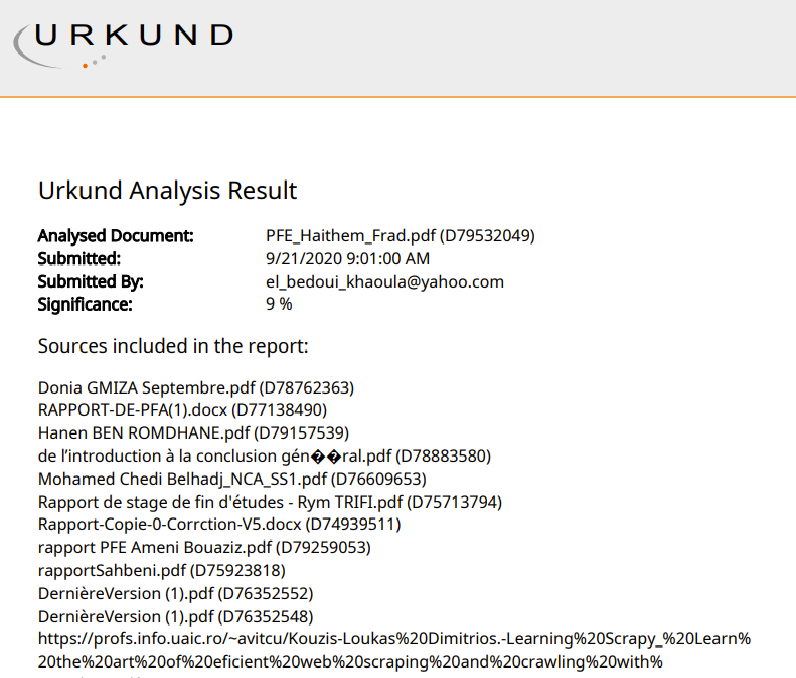
\includegraphics[width=0.95\columnwidth]{plagiat.png}}
    {\\\textbf{Figure annexe 2.1:} Rapport de Plagiat}
\end{figure}
